% You should title the file with a .tex extension (hw1.tex, for example)
\documentclass[12pt]{article}\sloppy

\usepackage{amsmath,bm}
\usepackage{amssymb}
\usepackage{fancyhdr}
\usepackage{graphicx}
\usepackage{float}
\usepackage{longtable}
\usepackage{hyperref}

\floatplacement{figure}{H}
\oddsidemargin0cm
\topmargin-2cm     %I recommend adding these three lines to increase the 
\textwidth16.5cm   %amount of usable space on the page (and save trees)
\textheight23.5cm  

\newcommand{\myname}{Abhinav Maurya}
\newcommand{\myandrew}{amaurya@andrew.cmu.edu}
\newcommand{\myhwnum}{5}

\newcommand{\question}[2] {\vspace{.25in} \hrule\vspace{0.5em} \noindent{\bf #1: #2} \vspace{0.5em} \hrule \vspace{.10in}}
\renewcommand{\part}[1] {\vspace{.10in} {\bf (#1)}}

\setlength{\parindent}{0pt}
\setlength{\parskip}{5pt plus 1pt}
 
\pagestyle{fancyplain}
\lhead{\fancyplain{}{\textbf{HW\myhwnum}}}      % Note the different brackets!
\rhead{\fancyplain{}{\myname\\ \myandrew}}
\chead{\fancyplain{}{16-720}}

\begin{document}

\medskip                        % Skip a "medium" amount of space
                                % (latex determines what medium is)
                                % Also try: \bigskip, \littleskip

\thispagestyle{plain}
\begin{center}                  % Center the following lines
{\Large 16-720: Assignment \myhwnum} \\
\myname \\
\myandrew \\
\end{center}

\question{1.1}{mygradient}

Included in \texttt{code/mygradient.m} file. Results in figure \ref{fig:1.1.1} and \ref{fig:1.1.2}.

\begin{figure*}[f]
\centering
\begin{tabular}{c c}
  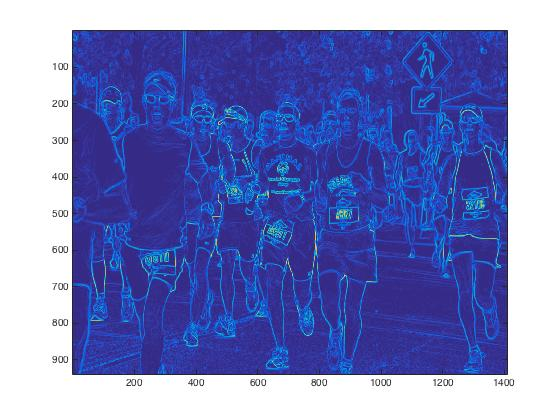
\includegraphics[width=0.45\linewidth]{fig1.jpg} & 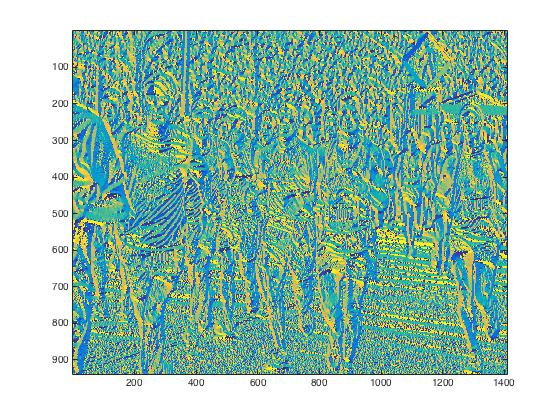
\includegraphics[width=0.45\linewidth]{fig2.jpg} \\
\end{tabular}
\caption{Magnitude and Orientation of Gradient on test0.jpg}
\label{fig:1.1.1}
\end{figure*}

\begin{figure*}[f]
\centering
\begin{tabular}{c c}
  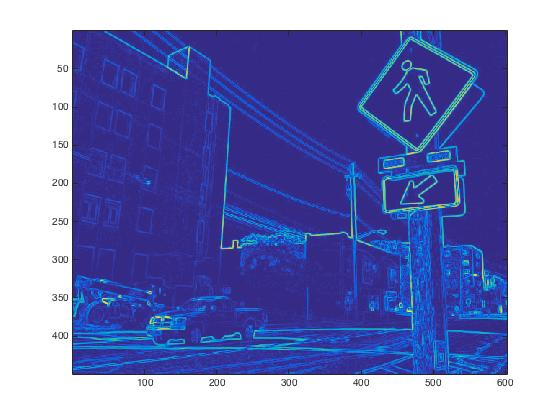
\includegraphics[width=0.45\linewidth]{fig3.jpg} & 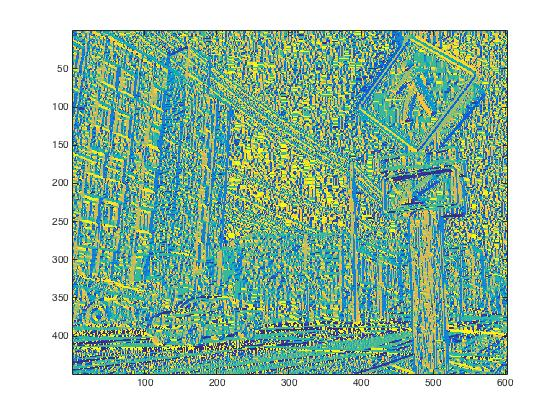
\includegraphics[width=0.45\linewidth]{fig4.jpg} \\
\end{tabular}
\caption{Magnitude and Orientation of Gradient on test1.jpg}
\label{fig:1.1.2}
\end{figure*}

\question{1.2}{hog}

Included in \texttt{code/hog.m} file. Results in figure \ref{fig:1.2.1}.

\begin{figure*}[f]
\centering
\begin{tabular}{c c}
  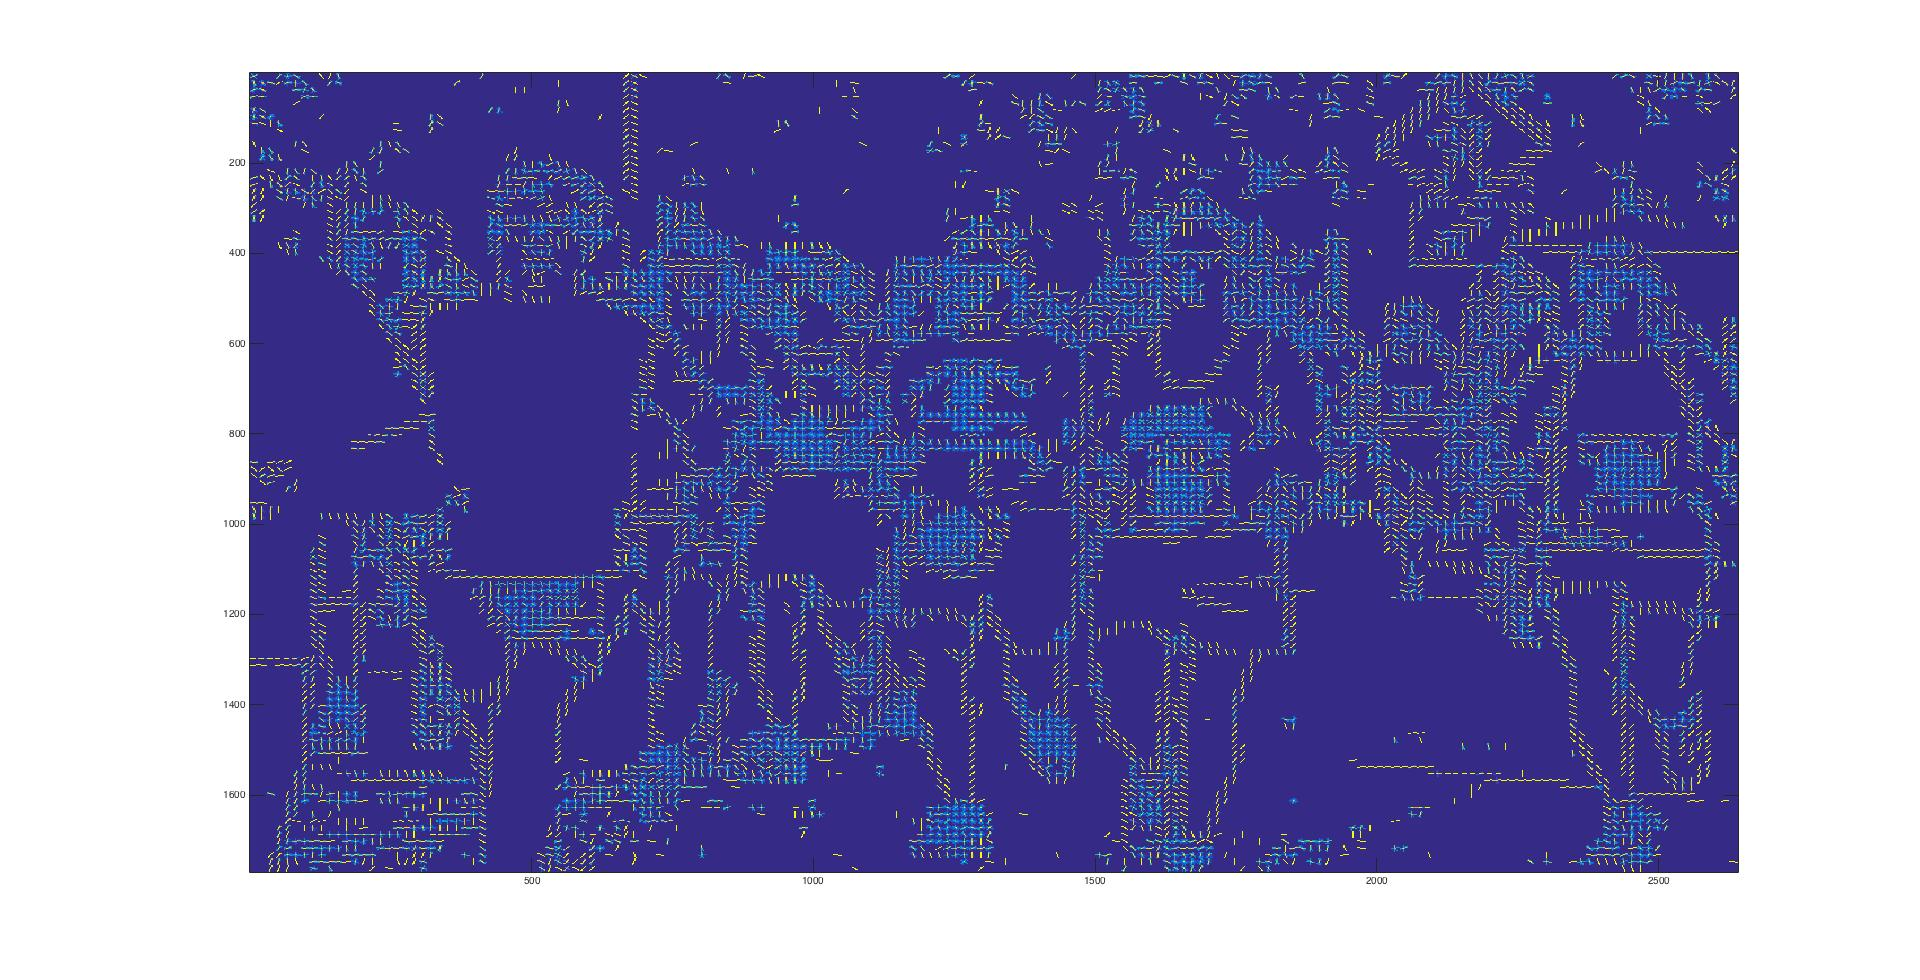
\includegraphics[width=0.45\linewidth]{fig5.jpg} & 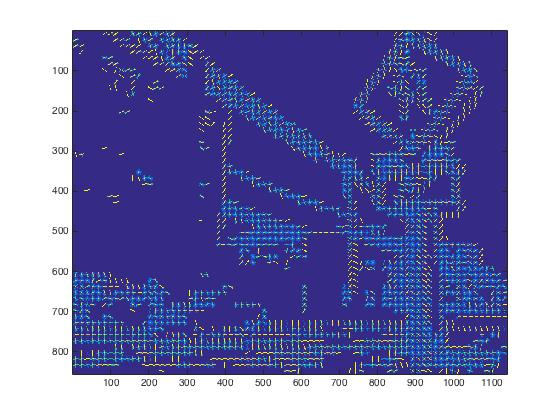
\includegraphics[width=0.45\linewidth]{fig6.jpg} \\
\end{tabular}
\caption{HOG Visualizations on test0.jpg and test1.jpg}
\label{fig:1.2.1}
\end{figure*}

\question{1.3}{detect}

Included in \texttt{code/detect.m} file. Results in figures \ref{fig:1.3.1} and \ref{fig:1.3.2}.

\begin{figure*}[f]
\centering
\begin{tabular}{c c}
  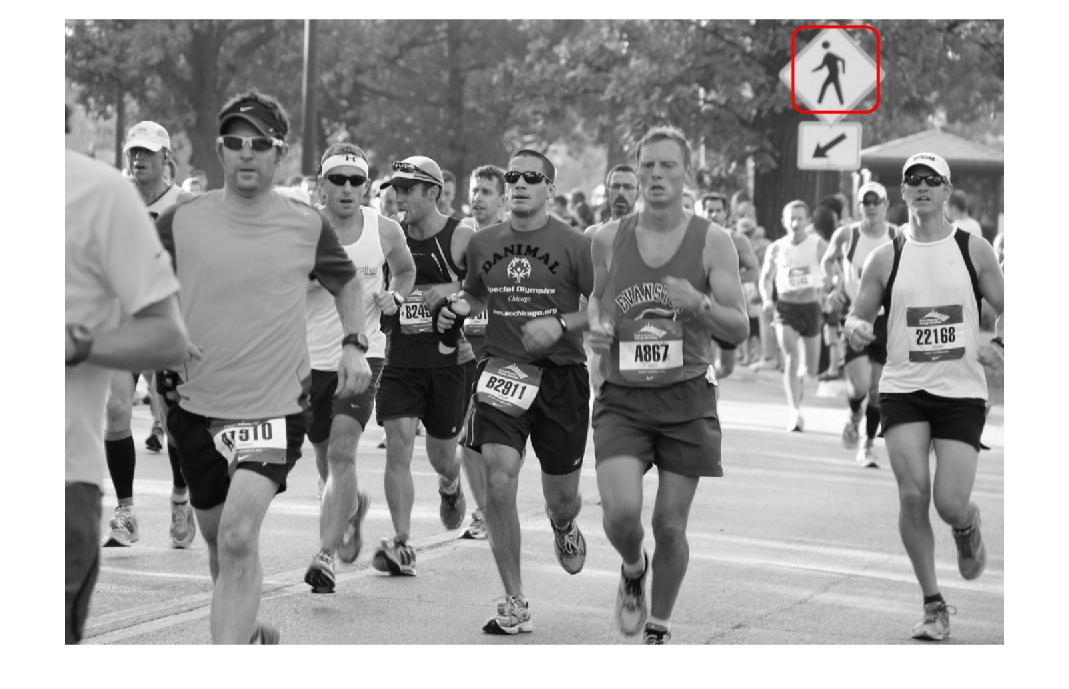
\includegraphics[width=0.45\linewidth]{fig12.jpg} & 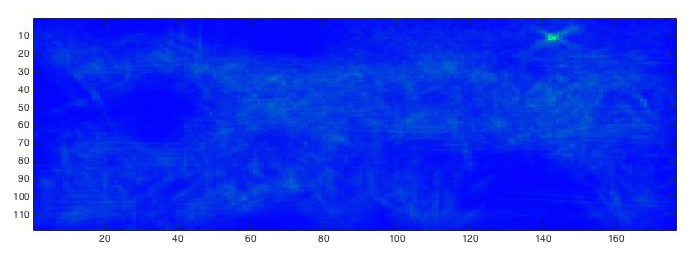
\includegraphics[width=0.45\linewidth]{fig8.jpg} \\
\end{tabular}
\caption{Cross-correlation and Detection on test0.jpg}
\label{fig:1.3.1}
\end{figure*}

\begin{figure*}[f]
\centering
\begin{tabular}{c c}
  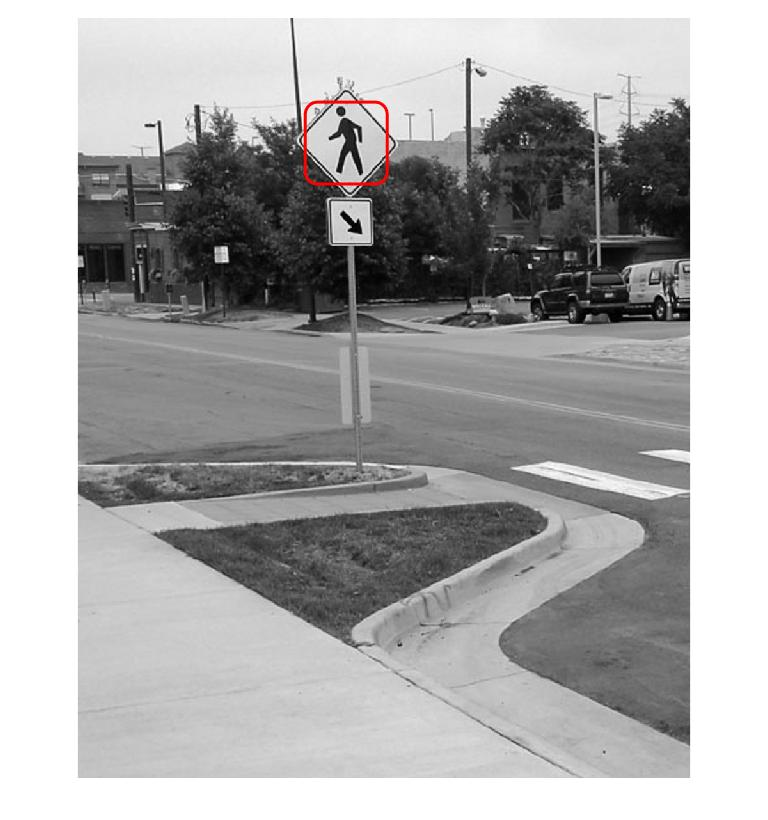
\includegraphics[width=0.45\linewidth]{fig13.jpg} & 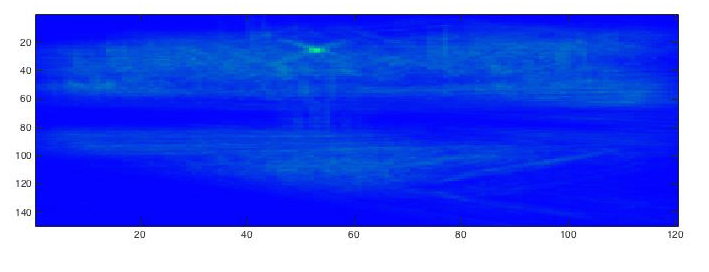
\includegraphics[width=0.45\linewidth]{fig14.jpg} \\
\end{tabular}
\caption{Cross-correlation and Detection on test4.jpg}
\label{fig:1.3.2}
\end{figure*}

\question{1.4}{Multiple Detections}

Included in \texttt{code/detect.m} file. Results in figure \ref{fig:1.4.1} and \ref{fig:1.4.2}.

\begin{figure*}[f]
\centering
\begin{tabular}{c c}
  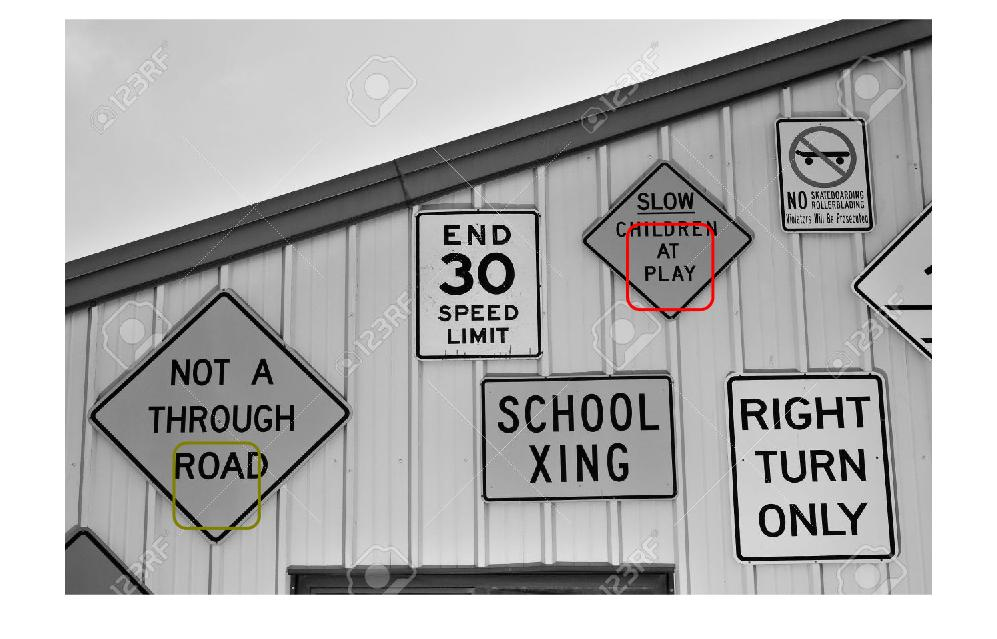
\includegraphics[width=0.45\linewidth]{fig15.jpg} & 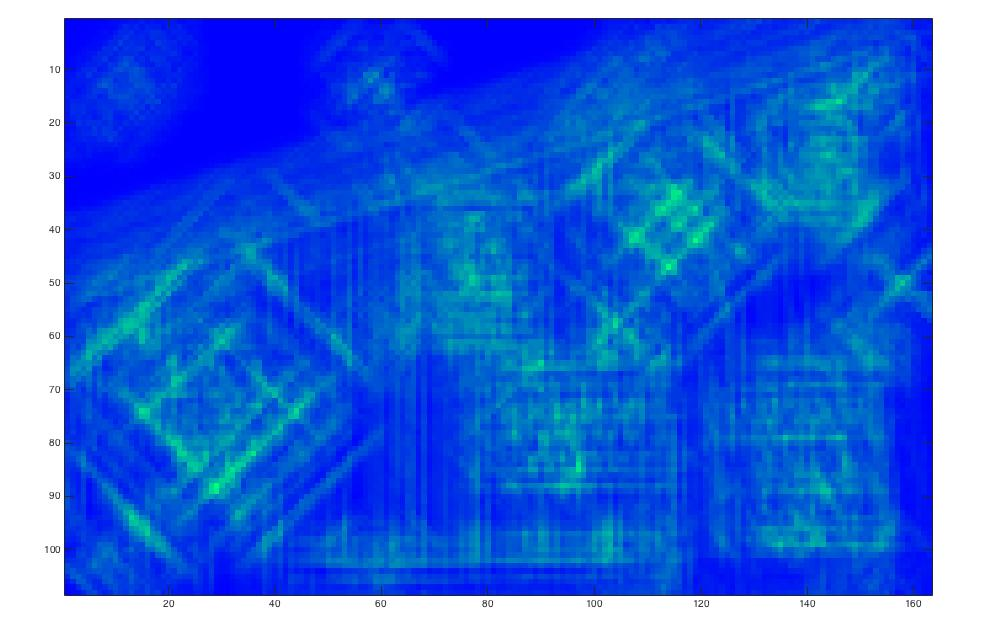
\includegraphics[width=0.45\linewidth]{fig16.jpg} \\
\end{tabular}
\caption{Cross-correlation and Detection on multiple-detections.jpg}
\label{fig:1.4.1}
\end{figure*}

\begin{figure*}[f]
\centering
\begin{tabular}{c c}
  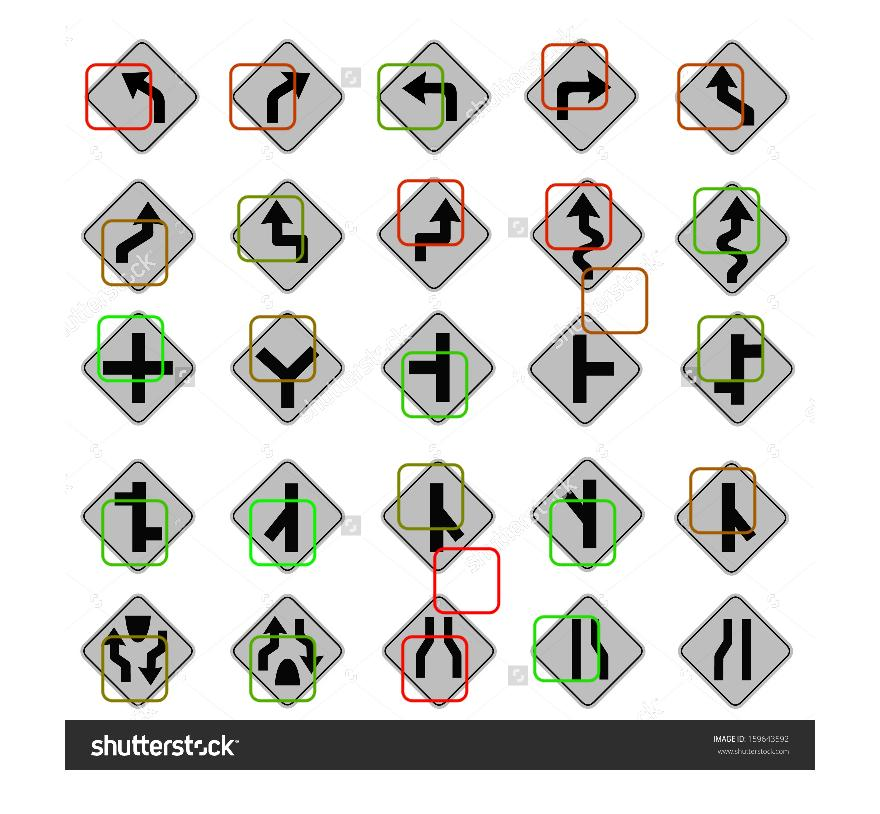
\includegraphics[width=0.45\linewidth]{fig9.jpg} & 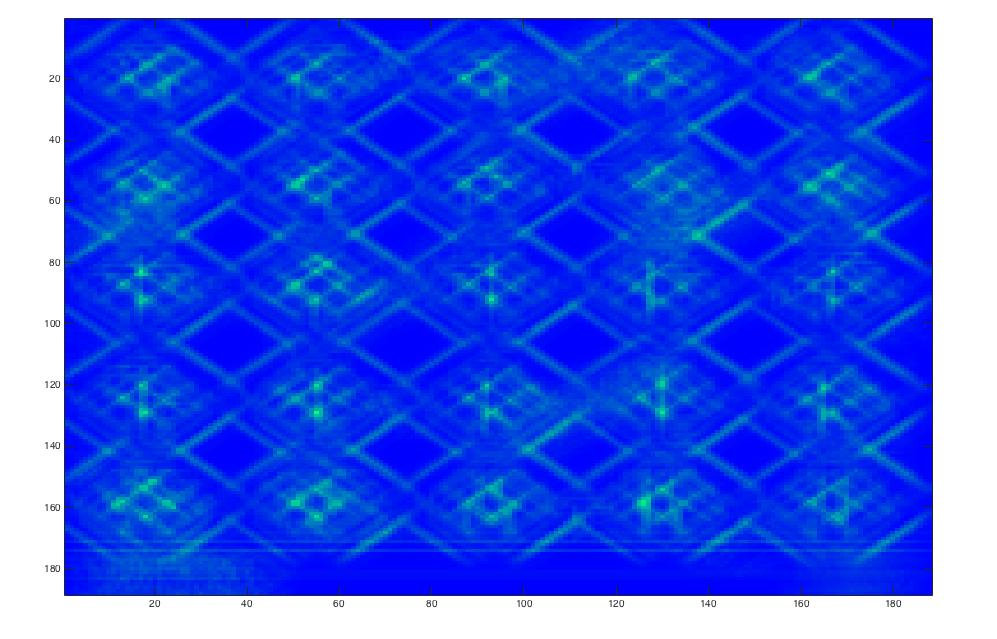
\includegraphics[width=0.45\linewidth]{fig11.jpg} \\
\end{tabular}
\caption{Cross-correlation and Detection on multiple-detections-extreme.jpg}
\label{fig:1.4.2}
\end{figure*}

\begin{figure*}[f]
\centering
\begin{tabular}{c c}
  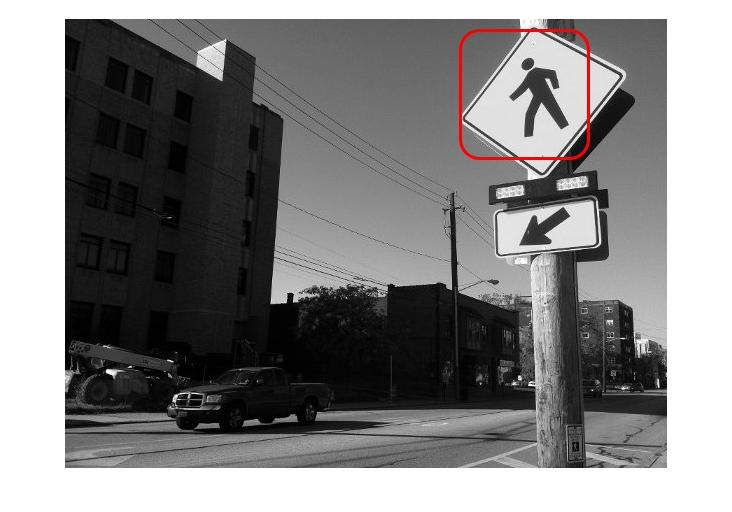
\includegraphics[width=0.45\linewidth]{fig20.jpg} & 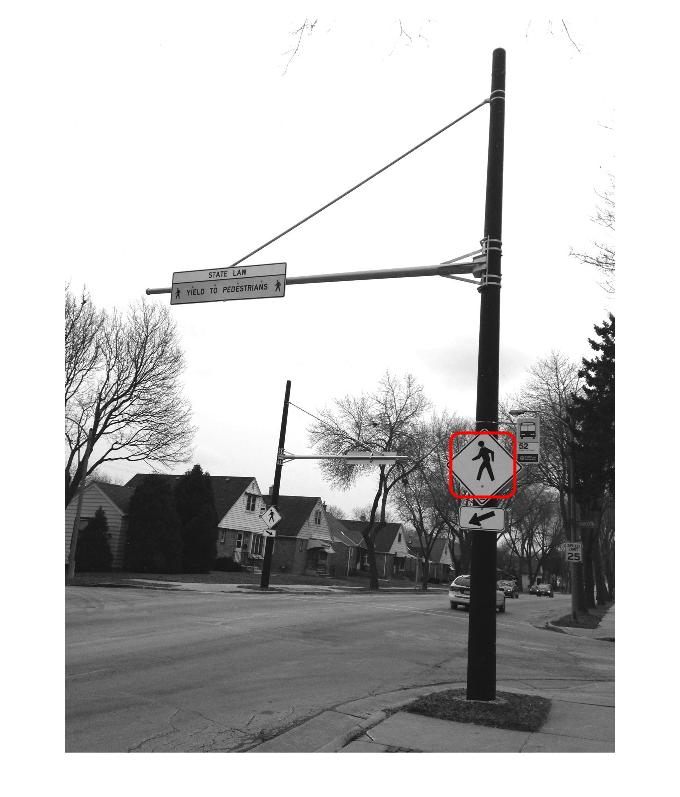
\includegraphics[width=0.45\linewidth]{fig21.jpg} \\
\end{tabular}
\caption{Detections on Test Images Provided}
\label{fig:1.3.3}
\end{figure*}

\question{2.1}{select\_patches}

Included in script \texttt{code/select\_patches.m} file. It displays multiple images. First, it displays all images with signs and then some control images without signs. The number of rectangles that can be selected per image are set in the script to 5. If there is a single traffic sign, I drew a bounding box around it multiple times so that the detector is given more examples and becomes tolerant to variances in the image and the exact position of the bounding box for the traffic signals.

\question{2.1}{tl\_pos}

Included in script \texttt{code/tl\_pos.m} file. Gets positive templates and averages them.

\question{2.2}{tl\_pos\_neg}

Included in script \texttt{code/tl\_pos\_neg.m} file. Subtracts the average of negative templates from the average of positive templates.

\question{2.3}{tl\_lda}

Included in script \texttt{code/tl\_lda.m} file. Subtracts the average of negative templates from the average of positive templates and premultiplies with the inverse of the covariance of negative templates as indicated in the handout. $\lambda=0.001$ was found to be robust in regularizing the low-rank or ill-conditioned nature of the covariance matrix.

\question{2.4}{multiscale\_detect}

Included in script \texttt{code/multiscale\_detect.m} file. Coded as directed in the assignment. Results in figures \ref{fig:2.4.1} and \ref{fig:2.4.2}. I found the tl\_pos\_neg template to work best, and therefore used it in the multiscale case.

\begin{figure*}[f]
\centering
\begin{tabular}{c}
  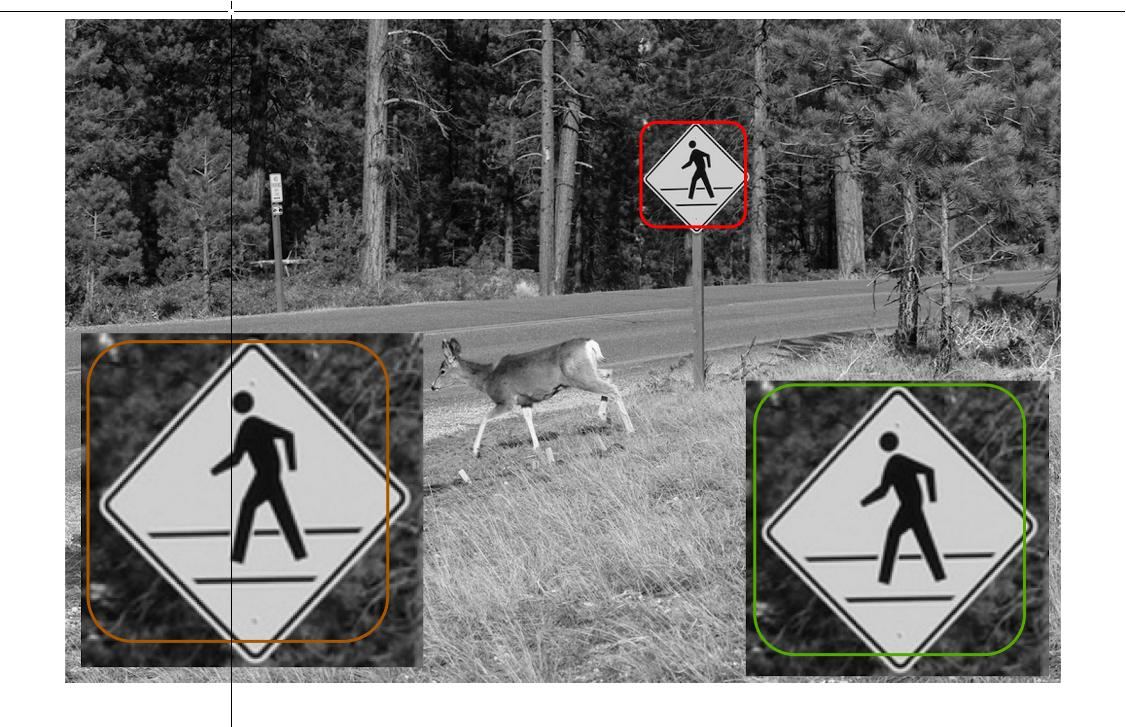
\includegraphics[width=0.45\linewidth]{fig19.jpg} \\
\end{tabular}
\caption{Multiple Detections at Different Scales}
\label{fig:2.4.1}
\end{figure*}

\begin{figure*}[f]
\centering
\begin{tabular}{c}
  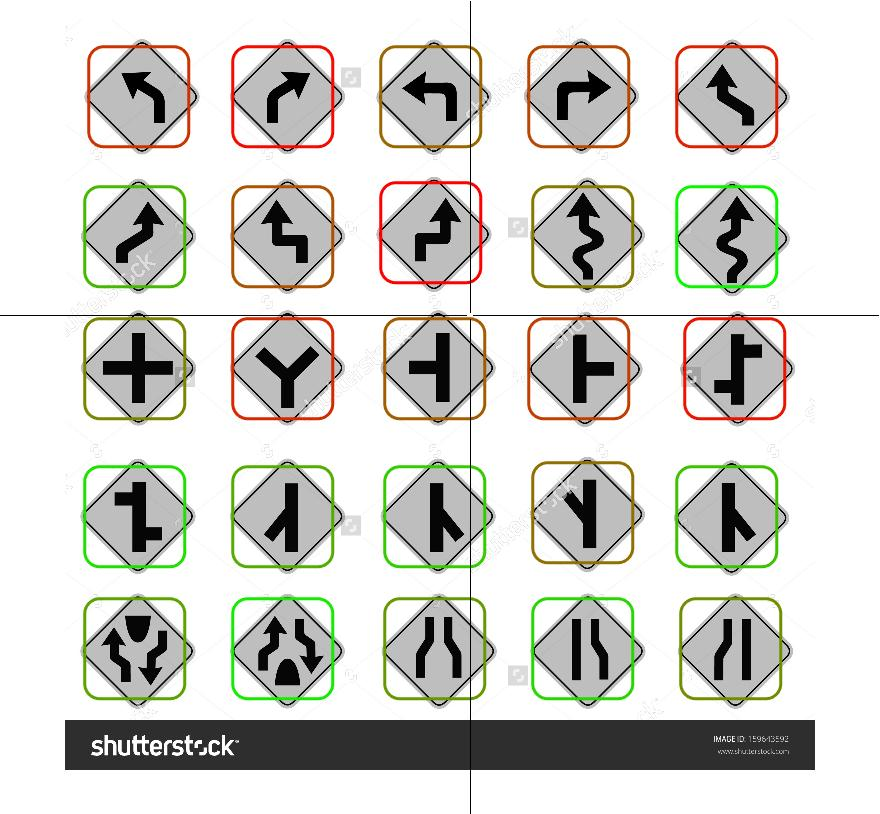
\includegraphics[width=0.45\linewidth]{fig17.jpg} \\
\end{tabular}
\caption{Multiple Detections of Traffic Signs at Same Scale}
\label{fig:2.4.2}
\end{figure*}

\begin{figure*}[f]
\centering
\begin{tabular}{c c c c c}
  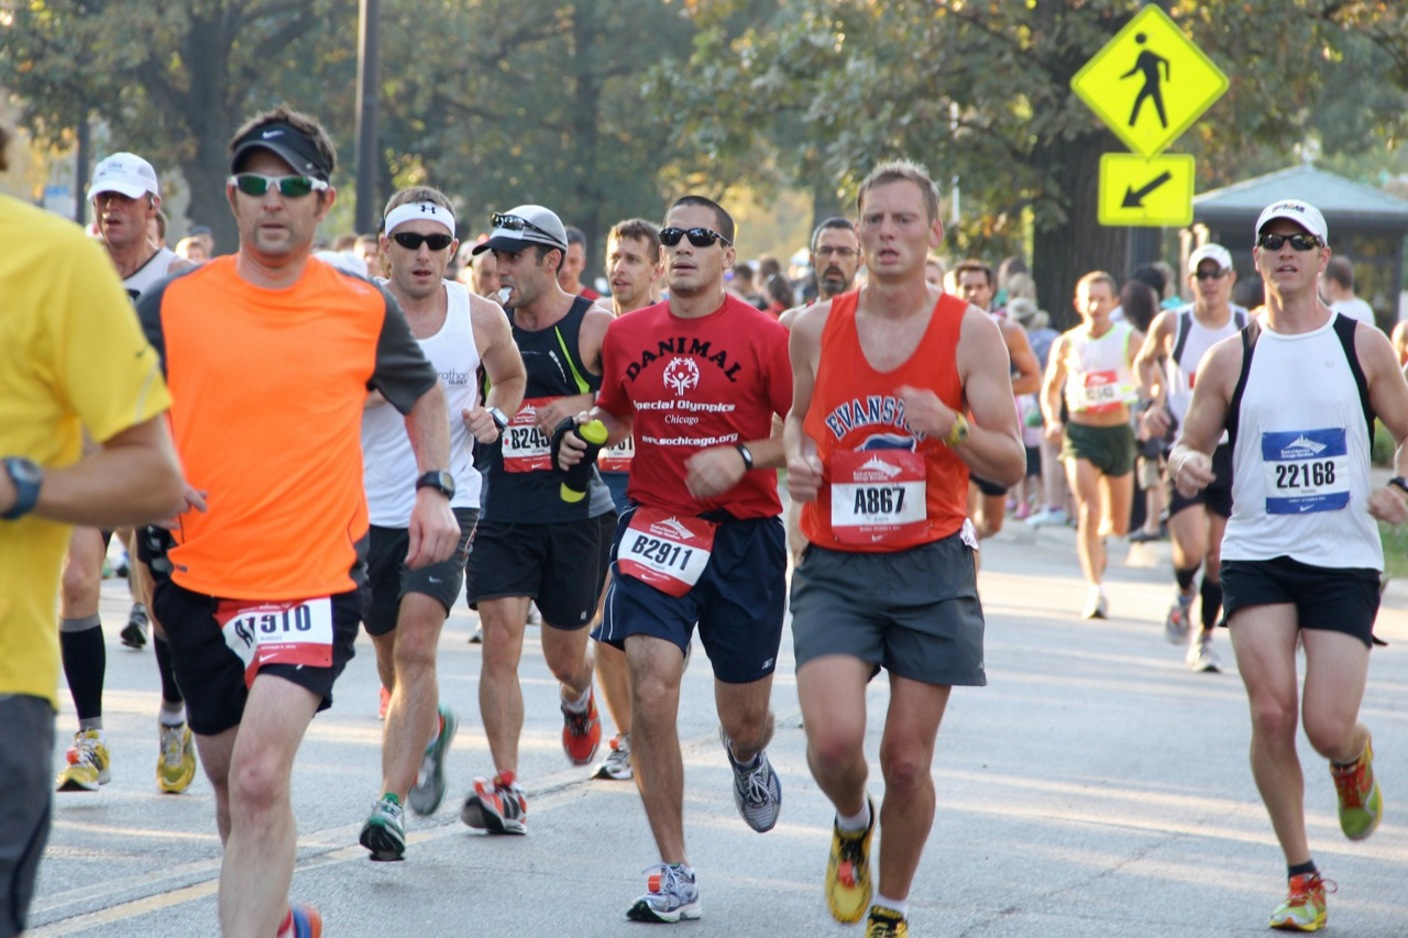
\includegraphics[width=0.18\linewidth]{../data/test0.jpg} & 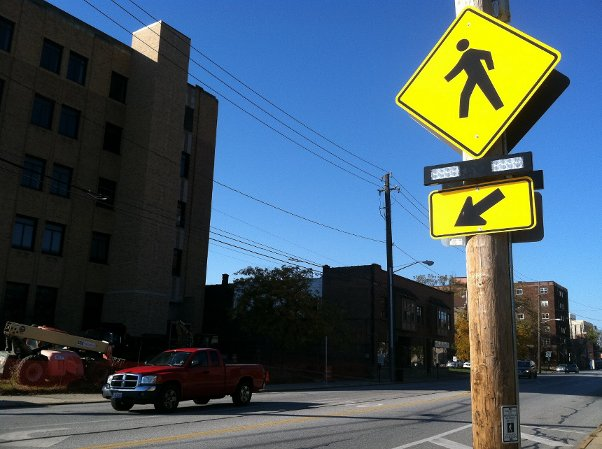
\includegraphics[width=0.18\linewidth]{../data/test1.jpg} &
  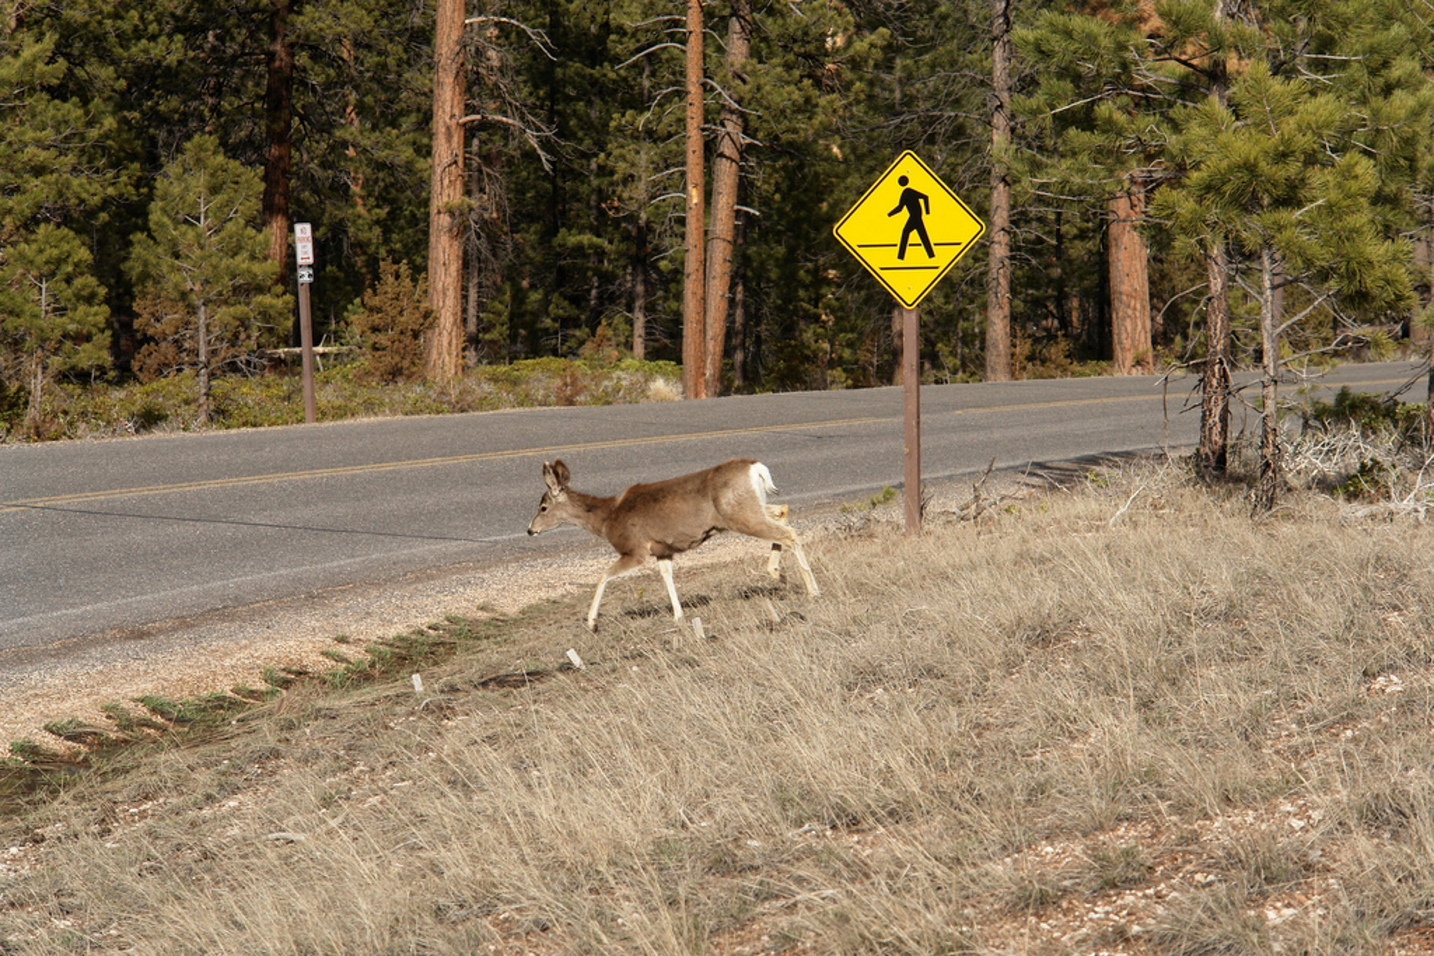
\includegraphics[width=0.18\linewidth]{../data/test2.jpg} & 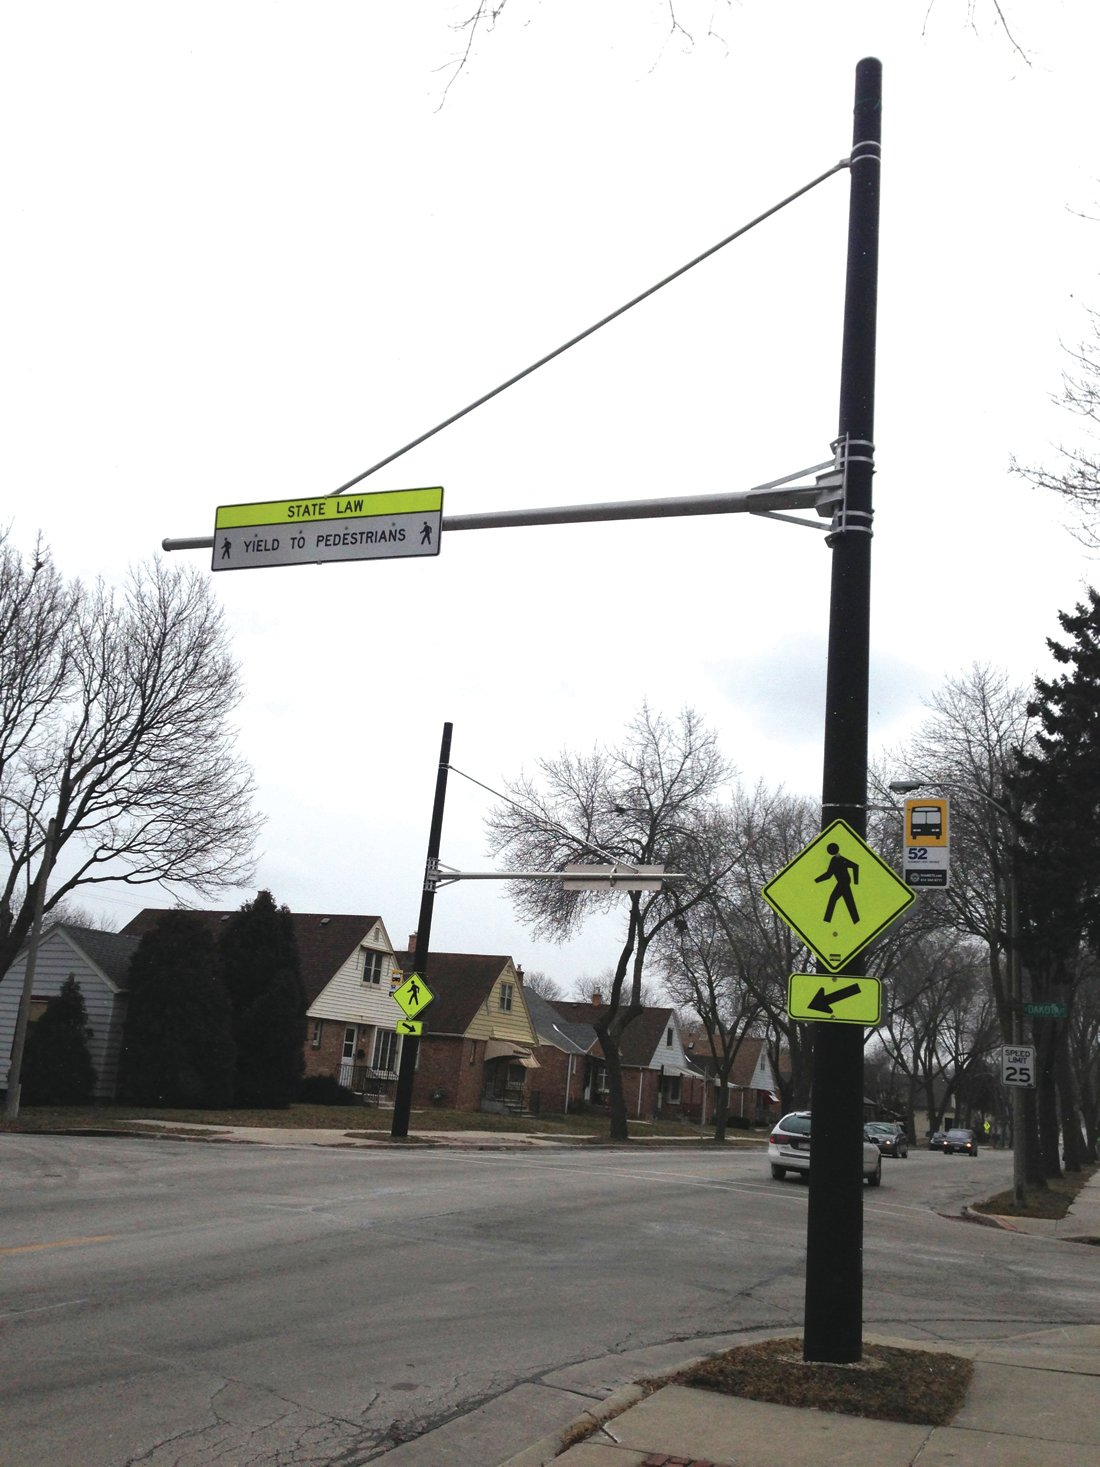
\includegraphics[width=0.18\linewidth]{../data/test3.jpg} &
  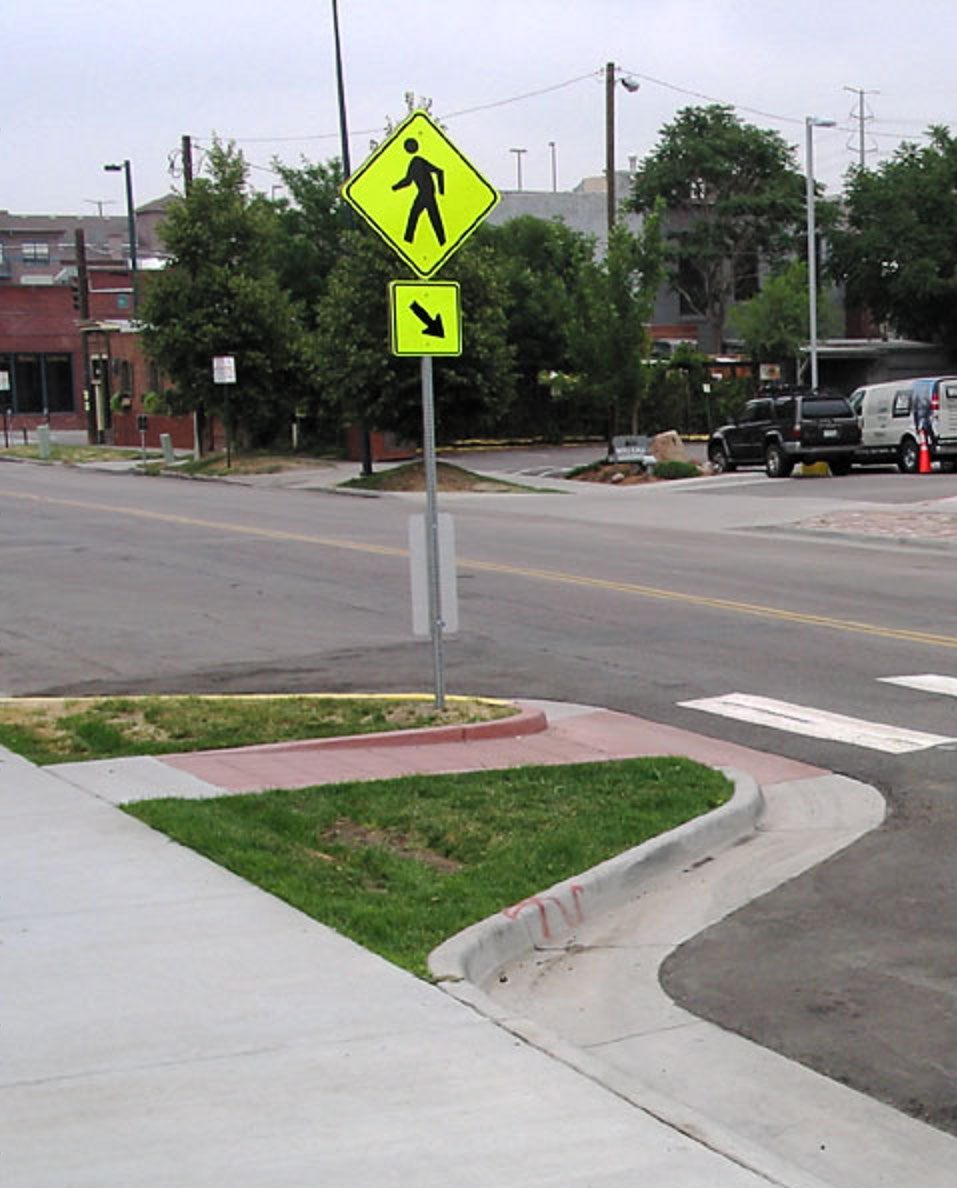
\includegraphics[width=0.18\linewidth]{../data/test4.jpg} \\
\end{tabular}
\caption{Positive Examples}
\label{fig:3.1}
\end{figure*}

\end{document}

